\documentclass[12pt,a4paper]{article}
\usepackage[utf8]{inputenc}
\usepackage{graphicx}
\usepackage{booktabs}
\usepackage{amsmath}
\usepackage{hyperref}
\usepackage{geometry}
\usepackage{float}

\geometry{margin=1in}

\title{%
  \textbf{P15: Sentiment Classification of IMDb Movie Reviews}\\
  \vspace{0.5em}
  \large CS485 -- Project Report
}
\author{%
  Zervos Spiridon Chrisovalantis (csd4878) \\
  Drakakis Rafail (csd5310)
}
\date{\today}

\begin{document}

\maketitle
\thispagestyle{empty}

\begin{abstract}
  We present an end-to-end pipeline for sentiment classification of the IMDb Movie Reviews dataset using both classical and deep learning techniques. We preprocess the data, extract features, train multiple models, and evaluate their performance. Classical ML models include Logistic Regression, Naive Bayes, and Linear SVM trained on TF–IDF vectors. Deep learning models include LSTM and 1D-CNN built using PyTorch with learned embeddings. We analyze accuracy, confusion matrices, and inference time. Our results show strong performance from classical methods, competitive CNN results, and poor LSTM learning without pretrained embeddings or tuning.
\end{abstract}

\newpage
\tableofcontents
\newpage

\section{Introduction}
Sentiment analysis seeks to classify text into categories such as positive or negative sentiment. The IMDb dataset offers a widely used benchmark of 50,000 labeled movie reviews. We compare two families of sentiment classification models:
\begin{itemize}
  \item \textbf{Classical ML}: Feature engineering with TF–IDF followed by Logistic Regression, Naive Bayes, and Linear SVM.
  \item \textbf{Deep Learning}: LSTM and CNN architectures with learned word embeddings and end-to-end training in PyTorch.
\end{itemize}

\section{Related Work}

Early approaches to movie‐review sentiment analysis relied on surface‐level representations such as bag‐of‐words and handcrafted lexicons. Pang and Lee demonstrated that simple unigram and bigram features fed into classical classifiers (e.g., Naïve Bayes, SVM) already achieved strong baselines on the IMDb dataset \cite{Pang2002}. Lexicon-based methods such as VADER and SentiWordNet leverage word‐level sentiment scores, offering interpretability but often struggling with context and negation.

The advent of distributed word embeddings (e.g., Word2Vec, GloVe) enabled neural models to capture semantic similarity. Kim popularized one-layer CNNs over word embeddings for sentence classification, showing that shallow convolutional filters can extract n-gram features effectively \cite{Kim2014}. Subsequent work introduced recurrent architectures—particularly LSTMs and GRUs—to model sequential dependencies and long-range context \cite{Tang2015}.

More recent studies incorporate hierarchical and attention-based mechanisms. Yang et al.\ proposed a Hierarchical Attention Network that applies attention at both word and sentence levels, improving document-level sentiment classification \cite{Yang2016}. The Transformer architecture introduced self-attention, laying the groundwork for large pretrained language models \cite{Vaswani2017}, and fine-tuning BERT and RoBERTa has since set new state‐of‐the‐art results on IMDb and related benchmarks \cite{Devlin2019, Liu2019}.

Finally, ensemble and hybrid methods—combining neural models with lexicon features or classical classifiers—have been shown to further boost robustness, particularly on noisy and out‐of‐domain data, motivating our exploration of contextual embeddings, attention layers, and ensemble strategies.

\section{Methodology}
\subsection{Dataset}
\begin{itemize}
  \item \textbf{Name:} IMDb Large Movie Review Dataset
  \item \textbf{Size:} 25,000 training and 25,000 test samples
  \item \textbf{Labels:} Binary sentiment – Positive (1), Negative (0)
  \item \textbf{Source:} \url{https://ai.stanford.edu/~amaas/data/sentiment/}
\end{itemize}

\subsection{Preprocessing}
\begin{itemize}
  \item Dataset is downloaded and extracted from Google Drive.
  \item Text normalization: lowercasing, tokenization (using NLTK \texttt{word\_tokenize}), removal of punctuation, numbers, and stopwords.
  \item For deep models: vocabulary built with a minimum frequency of 2 and capped at 20,000 tokens. Input sequences are padded or truncated to a maximum length of 200.
\end{itemize}

\subsection{Model Architectures \& Training Details}
\subsubsection{Classical Models}
\begin{description}
  \item[Logistic Regression:] $\ell_2$ regularization, $C = 1.0$, max\_iter = 1000
  \item[Multinomial Naive Bayes:] $\alpha = 1.0$
  \item[Linear SVM:] $C = 1.0$
\end{description}

\subsubsection{Deep Learning Models}
\begin{itemize}
  \item \textbf{Embedding Layer:} Embedding dimension = 100
  \item \textbf{LSTM:} Single-layer LSTM with 128 hidden units; classifier uses final hidden state
  \item \textbf{CNN:} 1D convolutions with filter sizes [3, 4, 5], 100 filters each; followed by max pooling and a fully connected layer
  \item \textbf{Training:} Optimized with Adam, learning rate = $1e^{-3}$, 5 epochs, batch size = 64
\end{itemize}

\section{Implementation}
\subsection{Preprocessing \& Vocabulary}
\begin{itemize}
  \item NLTK downloads handled programmatically for required packages: \texttt{punkt}, \texttt{punkt\_tab}, \texttt{stopwords}.
  \item Texts are lowercased, tokenized (using \texttt{word\_tokenize}), filtered for alphabetic words, and cleaned of English stopwords.
  \item For deep models: a vocabulary is built from training tokens with \texttt{min\_freq=2}, \texttt{max\_size=20000}. Sequences are padded or truncated to a fixed length of 200.
\end{itemize}

\subsection{Feature Extraction}
\begin{itemize}
  \item \textbf{Classical ML:} TF–IDF vectorization (unigrams only), limited to the top 5000 features.
  \item \textbf{Deep Learning:} Each word is mapped to a trainable embedding of dimension 100.
\end{itemize}

\subsection{Prediction Script}
A separate standalone script, \texttt{predict.py}, is provided for inference on new review texts using the trained CNN model.

\begin{itemize}
  \item \textbf{Architecture:} Re-implements the exact CNN Classifier architecture used during training.
  \item \textbf{Workflow:}
    \begin{enumerate}
      \item Loads the vocabulary from \texttt{vocab.pkl}.
      \item Loads the trained model weights from \texttt{model.pt}.
      \item Preprocesses the input review with the same tokenization and stopword removal.
      \item Converts the token sequence to indices and pads to length 200.
      \item Performs inference using PyTorch (CPU or CUDA).
      \item Outputs the predicted label (positive or negative) and the confidence score.
    \end{enumerate}
\end{itemize}

\section{Results \& Evaluation}
\subsection{Classical Machine Learning}

\begin{table}[H]
  \centering
  \caption{Accuracy and Inference Time (ms/sample) on 25,000 test samples}
  \label{tab:classical-summary}
  \begin{tabular}{lcc}
    \toprule
    \textbf{Model}          & \textbf{Accuracy} & \textbf{Time (ms/sample)} \\
    \midrule
    Logistic Regression     & 0.880             & 0.47                     \\
    Multinomial Naïve Bayes & 0.840             & 0.13                     \\
    Linear SVM              & 0.863             & 0.65                     \\
    \bottomrule
  \end{tabular}
\end{table}

\begin{table}[H]
  \centering
  \caption{Classification Report for Logistic Regression}
  \begin{tabular}{lcccc}
    \toprule
    \textbf{Class} & \textbf{Precision} & \textbf{Recall} & \textbf{F1-score} & \textbf{Support} \\
    \midrule
    Negative & 0.88 & 0.88 & 0.88 & 12500 \\
    Positive & 0.88 & 0.88 & 0.88 & 12500 \\
    \midrule
    \multicolumn{5}{l}{\textbf{Overall accuracy:} 0.88} \\
    \bottomrule
  \end{tabular}
\end{table}

\begin{figure}[H]
  \centering
  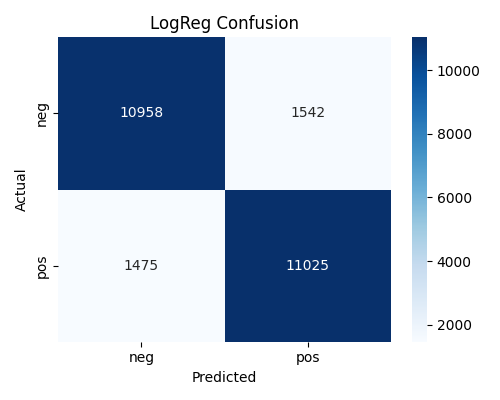
\includegraphics[width=0.6\textwidth]{figures/LogReg_confusion.png}
  \caption{Confusion matrix for Logistic Regression}
\end{figure}

\begin{figure}[H]
  \centering
  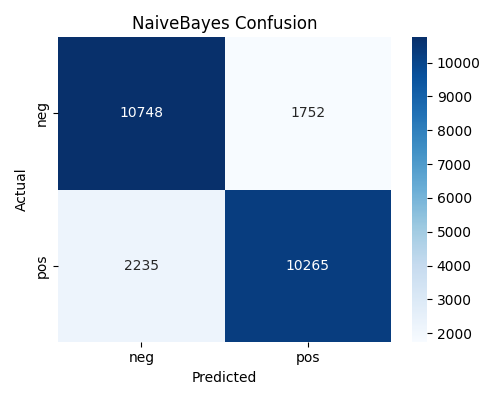
\includegraphics[width=0.45\textwidth]{figures/NaiveBayes_confusion.png}
  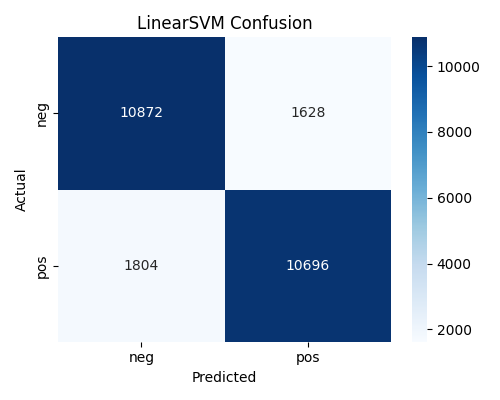
\includegraphics[width=0.45\textwidth]{figures/LinearSVM_confusion.png}
  \caption{Confusion matrices: Naïve Bayes (left), Linear SVM (right)}
\end{figure}

\subsection{Deep Learning}

\begin{table}[H]
  \centering
  \caption{Test Accuracy for Deep Models}
  \label{tab:dl-results}
  \begin{tabular}{lcc}
    \toprule
    \textbf{Model} & \textbf{Accuracy} & \textbf{Notes} \\
    \midrule
    LSTM & 0.511 & Underfitting, poor learning across epochs \\
    CNN  & 0.856 & Competitive with classical models \\
    \bottomrule
  \end{tabular}
\end{table}

\begin{figure}[H]
  \centering
  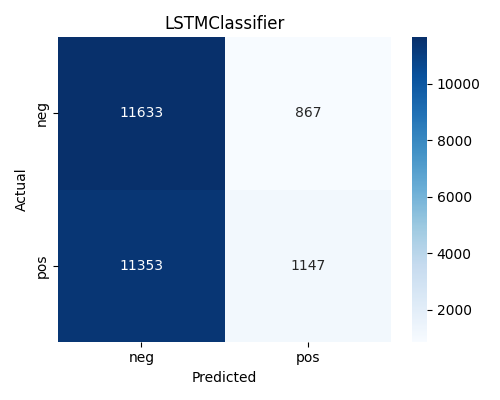
\includegraphics[width=0.45\textwidth]{figures/LSTMClassifier_confusion.png}
  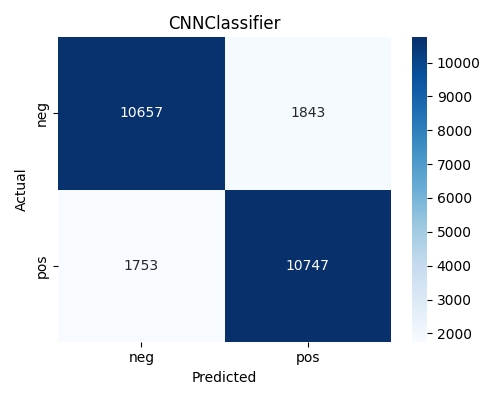
\includegraphics[width=0.45\textwidth]{figures/CNNClassifier_confusion.png}
  \caption{Confusion matrices: LSTM (left), CNN (right)}
\end{figure}

\section{Discussion}
\begin{itemize}
  \item \textbf{Inference speed:} Naïve Bayes is fastest (0.13ms/sample), followed by Logistic Regression (0.47ms), and Linear SVM (0.65ms).
  \item \textbf{Accuracy:} Logistic Regression is best overall (0.88), CNN comes close (0.856), and LSTM performs poorly (0.511).
  \item \textbf{Deep Learning Issues:}
    \begin{itemize}
      \item LSTM struggles due to lack of pretraining, insufficient data augmentation, and shallow architecture.
      \item CNN benefits from local n-gram pattern detection via convolution and max pooling.
    \end{itemize}
  \item \textbf{Generalization:} CNN is more robust than LSTM but needs GPU for fast training.
  \item \textbf{Short reviews:} Posed challenges for all models, especially with sarcasm or implicit sentiment.
\end{itemize}

\section{Conclusion \& Future Work}
\begin{itemize}
\item \textbf{Conclusion:} We implemented a full classification pipeline using classical and deep learning models for sentiment analysis on the IMDb dataset. Classical methods with TF–IDF and Logistic Regression remain strong baselines for accuracy and speed. While the CNN shows promising results, the LSTM architecture underperformed due to training instability and lack of optimization. Further improvements may include hyperparameter tuning, pretrained embeddings, and attention mechanisms.
\item \textbf{Future Work:} Future work could leverage pretrained transformers (e.g., BERT or RoBERTa) fine-tuned on your IMDb data and employ advanced augmentation (like back-translation) for greater robustness, alongside systematic hyperparameter search and regularization to stabilize training. Incorporating attention layers and ensembling neural and classical models can sharpen focus on key sentiment cues and exploit complementary strengths. Detailed error analysis with interpretability tools (e.g., LIME, SHAP) will uncover failure modes, while model compression (quantization, pruning) readies the pipeline for CPU-constrained deployment.
\end{itemize}

\begin{thebibliography}{9}

\bibitem{Pang2002}
Bo Pang, Lillian Lee, and Shivakumar Vaithyanathan. 2002. Thumbs up? Sentiment Classification using Machine Learning Techniques. In Proceedings of EMNLP 2002, pages 79–86. Association for Computational Linguistics. \url{https://aclanthology.org/W02-1011/}

\bibitem{Hutto2014}
C.~J. Hutto and E.~Gilbert. 2014. VADER: A Parsimonious Rule-based Model for Sentiment Analysis of Social Media Text. In Proceedings of the Eighth International Conference on Weblogs and Social Media (ICWSM-14). \url{https://ojs.aaai.org/index.php/ICWSM/article/view/14550}

\bibitem{Kim2014}
Yoon Kim. 2014. Convolutional Neural Networks for Sentence Classification. In EMNLP 2014. Association for Computational Linguistics. \url{https://aclanthology.org/D14-1181/}

\bibitem{Tang2015}
Duyu Tang, Bing Qin, and Ting Liu. 2015. Document Modeling with Gated Recurrent Neural Network for Sentiment Classification. Association for Computational Linguistics. \url{https://aclanthology.org/D15-1167/}

\bibitem{Yang2016}
Zichao Yang, Diyi Yang, Chris Dyer, Xiaodong He, Alex Smola, and Eduard Hovy. 2016. Hierarchical Attention Networks for Document Classification. Association for Computational Linguistics. \url{https://aclanthology.org/N16-1174/}

\bibitem{Vaswani2017}
Ashish Vaswani, Noam Shazeer, Niki Parmar, Jakob Uszkoreit, Llion Jones, Aidan N. Gomez, Łukasz Kaiser, and Illia Polosukhin. 2017. Attention Is All You Need.  (NeurIPS 2017). \url{https://papers.neurips.cc/paper/7181-attention-is-all-you-need.pdf}

\bibitem{Devlin2019}
Jacob Devlin, Ming-Wei Chang, Kenton Lee, and Kristina Toutanova. 2019. BERT: Pre-training of Deep Bidirectional Transformers for Language Understanding. Association for Computational Linguistics. \url{https://aclanthology.org/N19-1423/}

\bibitem{Liu2019}
Yinhan Liu, Myle Ott, Naman Goyal, Jingfei Du, Mandar Joshi, Danqi Chen, Omer Levy, Mike Lewis, Luke Zettlemoyer, and Veselin Stoyanov. 2019. RoBERTa: A Robustly Optimized BERT Pretraining Approach. \url{https://arxiv.org/abs/1907.11692}

\end{thebibliography}

\end{document}
